\documentclass[a4paper,12pt]{article}
\usepackage[left=78bp,right=78bp,top=68bp,bottom=62bp,footskip=28bp]{geometry}
\usepackage{fontspec,graphicx,array,colortbl,xurl}
\usepackage{amsmath,pgfplots}
\pgfplotsset{compat=1.18}
\definecolor{ink}{HTML}{293C44}
\definecolor{teal}{HTML}{286C78}
\definecolor{rust}{HTML}{AD563B}
\definecolor{ochre}{HTML}{A87327}
\pgfplotsset{every axis/.append style={font=\sffamily\footnotesize,
 axis lines*=left,axis line style={ink!55},tick style={ink!55},tick align=outside,
 tick label style={font=\sffamily\scriptsize,text=ink},
 label style={font=\sffamily\footnotesize,text=ink},
 legend style={font=\sffamily\scriptsize,text=ink,draw=none},
 title style={font=\sffamily\small\bfseries,text=ink},
 grid style={ink!13},major tick length=2pt}}
\usepackage[hidelinks]{hyperref}
\usepackage{xeCJK}
\setmainfont{Times New Roman}
\setCJKmainfont[BoldFont=SimHei,ItalicFont=KaiTi]{SimSun}
\setCJKsansfont[BoldFont=Microsoft YaHei Bold]{Microsoft YaHei}
\usetikzlibrary{arrows.meta}
\colorlet{sea}{teal}
\colorlet{clay}{rust}
\urlstyle{same}
\definecolor{tablegrey}{gray}{0.945}
\setlength\parindent{0pt}
\setlength\parskip{6bp}
\newcommand{\reportheading}[1]{{\fontsize{15bp}{19bp}\selectfont\bfseries #1\par}\vspace{4bp}}
\newcommand{\subhead}[1]{\par\addvspace{6bp}{\bfseries #1\par}\nobreak}
\newcommand{\reportfigure}[2]{\par\begingroup\centering #1\par{\fontsize{10bp}{12bp}\selectfont\itshape #2\par}\endgroup}
\newcommand{\tabletitle}[1]{\par{\fontsize{10bp}{12bp}\selectfont\bfseries #1\par}\nobreak}
\newcolumntype{L}[1]{>{\raggedright\arraybackslash}p{\dimexpr#1\linewidth-2\tabcolsep\relax}}
\newenvironment{reporttable}[1]{\par\begingroup\fontsize{10bp}{12bp}\selectfont\renewcommand{\arraystretch}{1.78}\begin{tabular}{#1}\hline}{\hline\end{tabular}\par\endgroup}
\newcommand{\tablenote}[1]{{\fontsize{10bp}{12bp}\selectfont #1\par}}
\newcommand{\referenceentry}[3]{\par\begingroup\raggedright\fontsize{11bp}{14bp}\selectfont\noindent\makebox[25bp][l]{[#1]}\begin{minipage}[t]{\dimexpr\linewidth-25bp\relax}\raggedright #2\par\noindent\url{#3}\end{minipage}\par\endgroup}
\makeatletter
\def\@oddfoot{\hfil{\fontsize{9bp}{10bp}\selectfont\thepage}\hfil}
\makeatother
\definecolor{pendingred}{rgb}{0.55,0.10,0.06}
\newcommand{\pendingdata}[1]{\par\smallskip\noindent\fcolorbox{pendingred}{white}{\parbox{\dimexpr\linewidth-2\fboxsep-2\fboxrule\relax}{\small\color{pendingred}\textbf{DATA PENDING}\quad #1}}\par}
\begin{document}
% Apply IEEEtran bibliography settings before the first reference.
\makeatletter
\immediate\write\@auxout{\string\citation{bibliography-control}}
\makeatother
\fontsize{11bp}{16bp}\selectfont
{\centering
{\fontsize{22bp}{26bp}\selectfont\bfseries 狭长房间的顶棚射流特性与排烟优化\par}
BSE3322 小型设计项目\quad 题目 B\par
{\fontsize{10bp}{13bp}\selectfont\textbf{第 18 组}\par
\begin{tabular}{@{}l@{\hspace{8pt}}l@{\hspace{26pt}}l@{\hspace{8pt}}l@{}}
HUANG Celine & 24034414D & LIU Wing Kei & 24093229D\\
LUO Qianyu & 24114977D & LYU Mingliang & 24099296D\\
WEN Jincheng & 24105273D & ZHUANG Wenyu & 24125669D
\end{tabular}\par}}
\medskip
\subhead{摘要}
即使顶棚排烟口能够捕集火源上方的烟气，狭长房间远端的烟层仍可能下降。本研究使用火灾动力学模拟软件（FDS），考察侧开口对顶棚射流温度的影响，并确定维持烟层净高所需的排烟量。与丙烷火实验对照发现，FDS 捕捉到了温度峰值向封闭侧偏移的趋势，温度误差的大小则随门态和火源功率而变化。针对丙烯火，我们在 16 个已有的挡烟垂壁与排烟量组合上，分别回放贝叶斯优化（BO）和遗传算法（GA）的搜索过程。两种算法均比固定顺序更早找到已测方案中净高余量最大的组合。随后，我们评估了改进布局，在顶棚设置两个排烟口，并按门态设定端墙补风口的高度。逐一用 FDS 计算六种门态与烟炱产率组合耗时较长，因此我们引入物理信息神经网络（PINN）快速预测各工况的最低烟层高度，并用已有 FDS 结果回放这一预筛策略，检验优先检查预测净高较低工况的效果。细网格 FDS 结果表明，1.12~m$^3$/s 是所测风量中满足约束且估算功率最低的选择。在六个工况各自的 120~s 模拟中，八个测点的最低烟层高度比 0.38~m 目标高出 55.8~mm。

\reportheading{1.\quad 引言}
火羽流撞击顶棚后，热气体沿顶棚向两侧流动。自然通风隧道的缩尺实验沿这一流动方向测量温度，记录顶棚射流随距离的衰减~\cite{tunnel}。在一侧设有多个门洞的狭长房间内，还需考虑补风从哪一侧进入。Peng 等~\cite{peng}在这一构型下改变侧门的开启组合，测量了顶棚温升沿房间长度的分布。他们的实验表明，羽流附近的温度取决于具体开启哪些门，随开口数量增加并无简单的变化规律。因此，沿房间纵向测得的温度剖面，可以同时检验模型对峰值温升及其位置的预测。

任务 1 利用 Peng 等的丙烷火实验，在四门全开和仅 R1 开启两种条件下检验上述特征。门口速度与温度剖面可用来判断冷空气从何处进入火源区、热气体从何处排出。顶棚机械排烟时，补充空气也沿这些通路进入房间。因此，任务 2 在两种门态下设计丙烯火排烟系统，针对不同门态预设端墙补风口，使两种门态与三种烟炱产率组合成的六个工况均保有 0.38~m 净高，并在所测风量中寻找功率最低者。我们回放原布局的设计搜索，并在改进布局中考察风量与工况的检查次序如何影响查询次数。风量推荐以 FDS 记录的最低烟层高度为依据。

\clearpage
\reportheading{2.\quad 研究方法}
两项任务均采用 Fire Dynamics Simulator 6.10.1（FDS）~\cite{fdsuser}。丙烷火沿用实验条件，用实测顶棚温升检验模型。丙烯火设计加入烟炱生成、顶棚机械排烟及补风，考察这些条件下房间能保有多少净高。

\reportfigure{\resizebox{.92\linewidth}{!}{\begin{tikzpicture}[font=\sffamily\large,text=ink,
 labelnode/.style={align=center,inner sep=3pt},
 title/.style={font=\sffamily\bfseries\large,align=center,inner xsep=9pt,inner ysep=3pt},
 flow/.style={draw=ink!85,line width=.85pt,-{Stealth[length=1.55mm]},rounded corners=2pt},
 stage/.style={draw=sea,line width=1.25pt,-{Stealth[length=1.75mm]}},
 tag/.style={font=\sffamily\normalsize,inner sep=2pt}]
% The stage bands carry the sequence; illustrations belong to their own stage.
\filldraw[draw=sea!30,fill=sea!6] (0,0) rectangle (15,-2.08);
\filldraw[draw=sea!30,fill=sea!4] (0,-2.94) rectangle (15,-5.05);
\filldraw[draw=ochre!40,fill=ochre!6] (0,-5.91) rectangle (15,-14.30);
\node[title,fill=sea!18] at (7.5,0) {房间与火源参数};
\node[title,fill=sea!18] at (7.5,-2.94) {任务 1\quad 丙烷火验证};
\node[title,fill=ochre!21] at (7.5,-5.91) {任务 2\quad 丙烯火排烟设计与优化};
\draw[stage] (7.5,-2.12)--(7.5,-2.61);
\draw[stage] (7.5,-5.09)--(7.5,-5.58);
% Physical plan and door states, simplified from the report's layout.
\begin{scope}[shift={(.66,-1.18)},x=.52cm,y=.52cm]
\filldraw[draw=ink,fill=white,thick] (0,0) rectangle (6.6,.9);
\foreach \x in {.825,2.475,4.125,5.775}
 \draw[sea,line width=2pt] (\x-.215,.9)--(\x+.215,.9);
\fill[clay] (3.175,.325) rectangle (3.425,.575);
\end{scope}
\node[labelnode] at (2.38,-1.66) {房间长度 6.60 m};
\foreach \y/\id in {-.74/OP-1,-1.16/OP-6}{
 \node[anchor=east,font=\sffamily\normalsize] at (6.83,\y) {\id};
 \foreach \k in {0,...,3}{\draw[ink!65,fill=white] (7+.42*\k,\y-.1) rectangle ++(.28,.20);}
}
\foreach \k in {0,...,3}{\fill[sea] (7+.42*\k,-.84) rectangle ++(.28,.20);}
\fill[sea] (7+.42*2,-1.26) rectangle ++(.28,.20);
\node[labelnode] at (7.50,-1.66) {侧门开启状态};
% Two burner symbols indicate the two prescribed heat release rates.
\foreach \x/\s in {11.73/.68,12.82/1}{
 \begin{scope}[shift={(\x,-1.24)},scale=\s]
 \draw[ink,line width=1.2pt] (-.31,0)--(.31,0);
 \fill[clay] (0,.04).. controls (-.53,.17) and (-.13,.51) ..(-.10,.65)
 .. controls (.05,.53) and (.11,.42) ..(.14,.30)
 .. controls (.23,.45) and (.23,.47) ..(.24,.52)
 .. controls (.50,.18) and (.26,.06) ..(0,.04);
 \end{scope}}
\node[labelnode] at (12.32,-1.66) {47.2 / 106.2 kW};
% Centre thumbnail uses the actual paired profile for OP-1 at 106.2 kW.
\begin{scope}[shift={(1.57,-4.21)},x=.33cm,y=.21cm]
\draw[step=1,sea!65,thin] (0,0) grid (5,2);
\draw[ink] (0,0) rectangle (5,2);
\draw[ink] (0,2)--(.7,2.85)--(5.7,2.85)--(5,2) (5.7,2.85)--(5.7,.85)--(5,0);
\end{scope}
\node[labelnode] at (2.52,-4.64) {运行四组 FDS};
\begin{axis}[at={(6.43cm,-4.25cm)},anchor=south west,scale only axis,width=2.08cm,height=.77cm,
 axis lines=left,axis line style={-,ink!55},xtick=\empty,ytick=\empty,xmin=0,xmax=660,ymin=250,ymax=1000]
\addplot[sea,thick] table[col sep=comma,x=sensor_x_cm,y=fds_rise_K]{../../05_Calculations/op1_106_coarse_90_120.csv};
\addplot[clay,only marks,mark=*,mark size=.85pt] table[col sep=comma,x=sensor_x_cm,y=exp_rise_K]{../../05_Calculations/op1_106_coarse_90_120.csv};
\end{axis}
\node[labelnode] at (7.48,-4.64) {对照 51 个测点};
\node[labelnode] at (12.45,-4.12) {比较不同门态下的\\峰值与温度剖面};
\draw[flow] (4.52,-4.07)--(5.59,-4.07);
\draw[flow] (9.33,-4.07)--(10.39,-4.07);

% The left lane follows physical design decisions. The right lane analyses FDS records.
\tikzset{designnode/.style={labelnode,font=\sffamily\small},
 decision/.style={designnode,draw=ochre!80,fill=white,rounded corners=2pt,inner sep=4pt}}
\draw[ochre!32] (8.42,-6.35)--(8.42,-13.97);
\node[designnode] (initial) at (2.23,-6.98) {\textbf{16 个 OP-6 方案}\\达标数 0/16};
\node[designnode] (layout) at (6.28,-6.98) {\textbf{调整布局}\\垂壁、排烟与补风};
\draw[flow] (initial.east)--(layout.west);
\node[designnode] (coarse) at (6.28,-8.47) {\textbf{FDS 粗网格筛选}\\0.96、1.28 通过};
\draw[flow] (layout.south)--(coarse.north);
\node[designnode] (refine) at (2.23,-8.47) {\textbf{加密竖向网格}\\复查净高};
\draw[flow] (coarse.west)--(refine.east);
\node[decision] (gate) at (2.23,-10.05) {\textbf{测试 1.12}\\OP-6，烟炱产率 0.02};
\draw[flow] (refine.south)--(gate.north);
\node[designnode] (six) at (6.28,-10.05) {\textbf{复核 1.12}\\两种门态，三种产率};
\draw[flow] (gate.east)--(six.west);
\node[designnode] (verified) at (2.23,-11.85) {\textbf{八个测柱，120 s}\\$h_{\min}=0.4358$ m};
\draw[flow] (six.south)--(six.south |- verified.east)--(verified.east);
\node[designnode,fill=white,draw=ochre!55,inner sep=5pt] (power) at (4.16,-13.42)
 {$\displaystyle\min P$\quad s.t.\ 各测点净高 $\geq0.38$ m\\
 \textbf{选择 1.12 m$^3$/s}\quad 6.91 W；1.28 为 10.32 W};
\draw[flow] (verified.south)--(verified.south |- power.north);
\node[designnode,text=sea] (replay) at (11.82,-6.67) {\textbf{回放同组 16 个方案}};
\draw[flow] (initial.north)--++(0,.30)-|(8.72,-6.67)--(replay.west);
\foreach \x/\heading/\ranks in {
 10.25/{贝叶斯优化}/{1,9,12,2,10,16,5,11,14,6,15,7,3,13,8,4},
 13.22/{遗传算法}/{1,13,8,2,14,10,9,5,15,16,7,6,3,12,11,4}}{
 \node[align=center,font=\sffamily\normalsize] at (\x,-7.36) {\heading};
 \foreach \q [count=\i from 0] in \ranks{
  \pgfmathtruncatemacro{\rownum}{int(\i/4)}
  \pgfmathtruncatemacro{\colnum}{mod(\i,4)}
  \begin{scope}[shift={(\x+.42*\colnum-.63,-7.99-.34*\rownum)}]
   \ifnum\i=11
    \fill[sea] (-.21,-.17) rectangle (.21,.17);
    \node[text=white,font=\sffamily\bfseries\small] {\q};
   \else
    \filldraw[draw=ink!24,fill=white,line width=.3pt] (-.21,-.17) rectangle (.21,.17);
    \node[font=\sffamily\small] {\q};
   \fi
  \end{scope}}
}

\node[designnode] at (11.82,-9.83) {查到最大余量\\固定 16 \quad BO 7 \quad GA 6--11};
\node[designnode] (hist) at (11.82,-11.04) {\textbf{已归档 FDS 最低净高}};
\node[designnode] (pred) at (11.82,-12.18) {\textbf{PINN 与回归}\\预测候选方案最低净高};
\node[designnode,text=sea] (test) at (11.82,-13.53) {以留出 FDS 结果\\检验预筛精度};
\draw[flow] (hist.south)--(pred.north);
\draw[flow] (pred.south)--(test.north);
\draw[flow,draw=sea] (pred.west)--(8.80,-12.18)--node[pos=.48,above,sloped,font=\sffamily\small,text=sea]{建议检查顺序}(8.80,-8.47)--(coarse.east);
\end{tikzpicture}
}}{左栏为 FDS 筛选和风量决策。右栏为两项独立分析：BO/GA 回放设计顺序，代理模型预估工况最低净高。风量单位为 m$^3$/s。蓝绿色单元格标出回放中净高余量最大的方案（GA 示意采用随机种子 0）。回箭头表示可用代理模型安排未来 FDS 的检查顺序。}


\subhead{2.1\quad 任务 1：丙烷火与顶棚射流验证}
房间尺寸取自题目 B 任务书图 1 和 Peng 等的实验~\cite{peng}。模型内部长、宽、高分别为 $6.60\times0.90\times0.76$~m，地面正中的正方形燃烧器边长 0.25~m，中心位于 $x=3.30$~m。同一侧墙上设四个门洞，沿 $x$ 递增方向依次为 L2、L1、R1 和 R2，各宽 0.43~m、高 0.63~m。计算域从这面墙向外延伸至 $y=1.40$~m，使空气可以从同一门洞的不同高度进出。参考环境温度为 $27.5\,^{\circ}$C。

第 18 组在四门全开（OP-1）和仅开 R1（OP-6）时，各自计算 47.2 和 106.2~kW 两档名义热释放率。FDS 按单位燃烧器面积指定热释放率，燃烧器边缘对齐网格面后，实际占地面积可能随网格改变。因此，每次换网格都核对燃烧器面积，并检查计算中记录的热释放率。

\clearpage
\subhead{空间分辨率与物理子模型}
OP-1 在相同计算域中采用 $132\times28\times19$、$176\times36\times25$ 和 $220\times48\times32$ 三种网格。按 FDS 用户指南~\cite{fdsuser}，火源特征直径为
\[
 D^*=\left(\frac{\dot Q}{\rho_\infty c_p T_\infty\sqrt{g}}\right)^{2/5}.
\]
式中 $\dot Q$ 为名义火源功率，$g$ 为重力加速度，$\rho_\infty$、$c_p$ 和 $T_\infty$ 分别为环境空气的密度、比热容和绝对温度。以 $D^*$ 除以单元最长边，可比较各网格对火源的分辨能力。再对照各网格算出的纵向温升剖面，判断加密对结果的影响。

\subhead{任务 1：控制变量对照与实验测量}
在 OP-1、106.2~kW 的粗网格上，先将辐射份额固定为 0.29，比较 Deardorff 与 WALE 两种亚网格模型~\cite{fdstech}。Yuen 等也在房间火灾模拟中考察过模型选择的影响~\cite{yuen}。随后保留 Deardorff，将辐射份额分别调至 0.20 和 0.50。壁面散热另作成对比较，将绝热壁换成 15~mm 导热板。板厚取自 Peng 等的实验~\cite{peng}，密度 200~kg/m$^3$、导热系数 0.10~W/(m\,K) 和比热容 1.0~kJ/(kg\,K) 则借用 FDS Steckler 第 10 号算例的保温材料参数~\cite{steckler}。OP-6 的两种壁面均用 $154\times56\times23$ 门流诊断网格。47.2~kW 的 OP-1 对照均用原粗网格。

从 Peng 等~\cite{peng}图 9 的顶棚纵向温升曲线读取 51 个位置，与模型中 $z=0.74$~m 处的 1~mm 热电偶逐点配对。对位置 $i$，按设备实际输出间隔求 90--120~s 内的时间加权平均温度，再减去模型环境温度，即得该点的模拟温升。取 $e_i=\Delta T_{\mathrm{FDS},i}-\Delta T_{\mathrm{exp},i}$，则整条剖面的平均偏差和均方根误差分别为
\[
 \mathrm{bias}=\frac{1}{51}\sum_{i=1}^{51}e_i,\qquad
 \mathrm{RMSE}=\sqrt{\frac{1}{51}\sum_{i=1}^{51}e_i^2}.
\]
另记录最热测点相对燃烧器中心的位置，以判断峰位是否偏移。同一时段内，R1 门口的速度和温度剖面给出各高度的进出流向和气流温度。将门流结果与壁面、辐射对照结合，可分析门洞输运与围护结构散热对顶棚温升的影响。

\subhead{房间平面与排烟布局}
\reportfigure{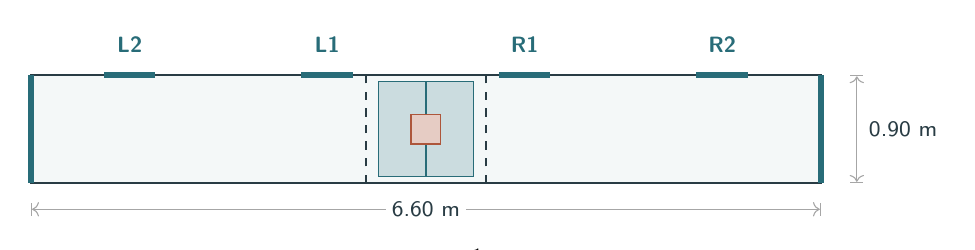
\begin{tikzpicture}[x=1.52cm,y=1.52cm,font=\sffamily\footnotesize]
\fill[teal!5] (0,0) rectangle (6.6,.9);
\draw[ink,line width=.7pt] (0,0) rectangle (6.6,.9);
\foreach \x/\id in {.825/L2,2.475/L1,4.125/R1,5.775/R2}{
 \draw[white,line width=2.3pt] (\x-.215,.9)--(\x+.215,.9);
 \draw[teal,line width=2pt] (\x-.215,.9)--(\x+.215,.9);
 \node[above,text=teal] at (\x,1.01){\bfseries \id};}
\filldraw[fill=teal!24,draw=teal] (2.9,.05) rectangle (3.3,.85);
\filldraw[fill=teal!24,draw=teal] (3.3,.05) rectangle (3.7,.85);
\foreach \x in {2.8,3.8}{\draw[ink,dashed,thick] (\x,0)--(\x,.9);}
\filldraw[fill=rust!30,draw=rust] (3.175,.325) rectangle (3.425,.575);
\foreach \x in {0,6.6}{\draw[teal,line width=2.4pt] (\x,0)--(\x,.9);}
\draw[gray!70,|<->|] (0,-.22)--node[fill=white,inner sep=2pt,text=ink]{6.60 m}(6.6,-.22);
\draw[gray!70,|<->|] (6.90,0)--(6.90,.9);
\node[right,text=ink] at (6.92,.45){0.90 m};
\end{tikzpicture}\par
{\sffamily\footnotesize\textcolor{rust}{\rule{6pt}{6pt}} 燃烧器\qquad
\textcolor{teal!65}{\rule{6pt}{6pt}} 顶棚排烟口\qquad
\textcolor{ink}{-- --} 挡烟垂壁\qquad\textcolor{teal}{\rule[.4ex]{10pt}{1.6pt}} 开口}}{名义几何的平面图。丙烷火模型使用图示侧开口。丙烯火设计增加端墙补风口，并在燃烧器上方两道挡烟垂壁之间设置两个顶棚排烟口。}

\clearpage
\subhead{2.2\quad 任务 2：丙烯火与排烟设计}
丙烯火的名义热释放率为 106.2~kW。基准烟炱产率取 0.02~kg/kg 燃料，CO 产率取 0.01~kg/kg。另将烟炱产率提高至 0.05 和 0.10~kg/kg，CO 产率保持原值。每种烟炱产率分别计算 OP-1 和 OP-6，共六个工况，每次计算中门的开闭状态固定。原设计网格为 $132\times28\times19$，围护结构表面按绝热处理。

\subhead{候选方案筛选与布局调整}
两次回放回答不同的检查次序问题。原布局中，BO 和 GA 根据此前查到的 FDS 余量选择下一个设计。改进布局中，PINN 等模型根据已有 FDS 数据预测最低净高，决定同一风量下先查哪个工况。最终选取风量时，逐一核查六个工况的完整 FDS 记录。

最初在 OP-6、基准烟炱产率下，将四种挡烟垂壁下垂深度（0、0.08、0.16、0.24~m）与四种总排烟量（0.08、0.16、0.24、0.32~m$^3$/s）交叉组合。固定顺序、贝叶斯优化（BO）~\cite{bo} 和遗传算法（GA）~\cite{ga} 均从同样的四个角点设计开始。每次查询揭示一个已归档的 FDS 余量，BO 和 GA 仅使用当时已揭示的余量选择下一设计。统计首次发现最大已记录余量所需的全部查询次数，GA 使用 20 个随机种子重复回放。

改进布局从两侧端墙的近地面开口补风。开口下缘与地面齐平，OP-1 时开至 0.44~m，OP-6 时开至 0.48~m。燃烧器正上方设两个顶棚排烟口，各接一条独立支管。两道横向挡烟垂壁位于排烟口两侧，分别设在 $x=2.8$ 和 3.8~m 处，自顶棚下垂 0.24~m。

\reportfigure{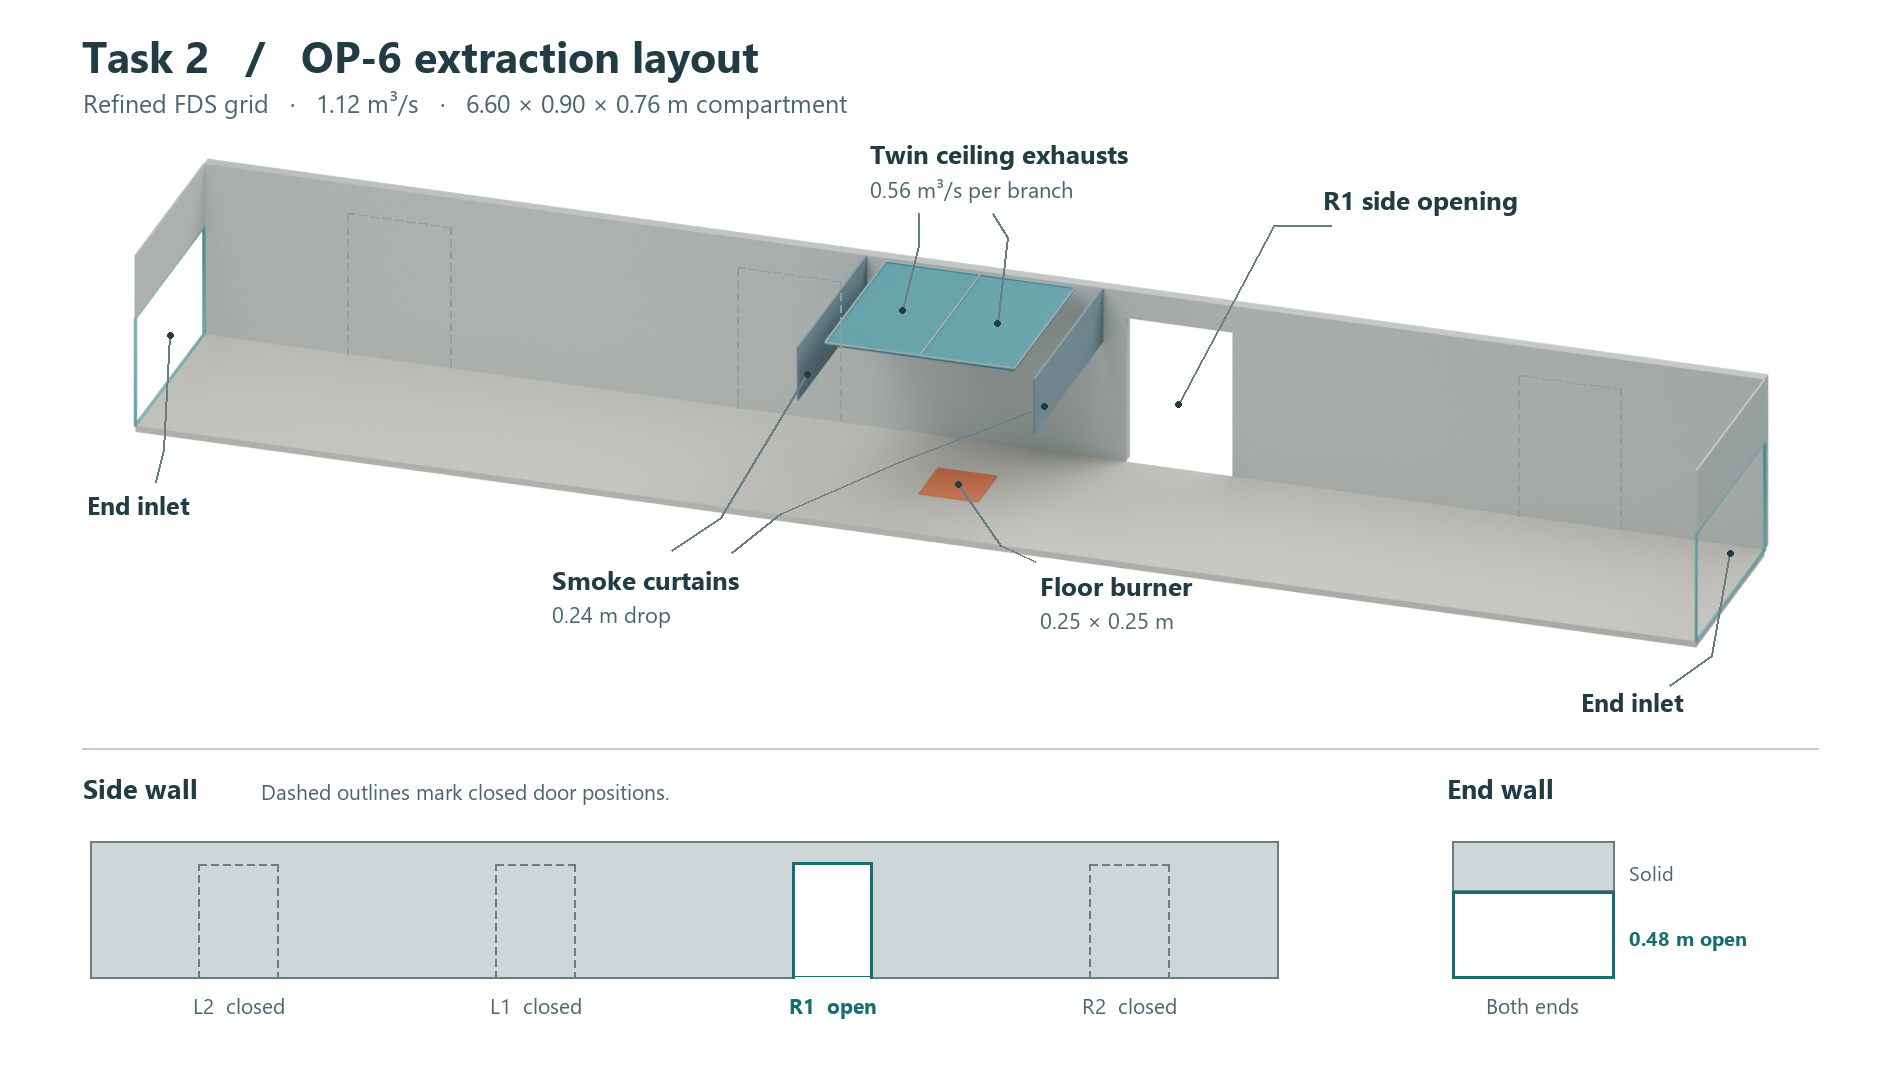
\includegraphics[width=\linewidth]{../figures/op6_1p12_fds_geometry_review.png}}{OP-6 改进布局的细网格剖视图。为展示室内构件，图中剖去近侧墙。FDS 中该处（$y=0$）为连续绝热墙面。侧墙只开启 R1，虚线标出关闭的三个门位。两端墙各设一个从地面起高 0.48~m 的补风口。}

按上述高度设置补风口，两条排烟支管均分总风量。先在六个工况下比较 0.96 和 1.28~m$^3$/s，再加密竖向网格，测试中间一档 1.12~m$^3$/s。另作工况排序回放时，将上述补风布局整类留出，不参与训练。物理信息神经网络（PINN）在拟合观测数据时可加入物理方程的残差约束~\cite{pinn}。三个风量按功率递增检查，每个风量下按 PINN、直接回归或二者等权平均预测的净高排序，先查预测最低的工况（第 5.2 节）。

\subhead{烟层高度判据与局部烟气测量}
FDS 在中央纵剖面 $y=0.45$~m 上布置八列竖向测点，根据温度推算烟层高度 $h_j(t)$。沿房间纵向的位置为 0.5、1.7、2.4、3.0、3.6、4.2、4.9 和 6.1~m。设备名义采样间隔为 0.5~s。工况 $s$ 的采样净高余量为
\[
 m_s=\min_{j,\,0\leq t\leq120\,\mathrm{s}} h_{j,s}(t)-0.38\,\mathrm{m}.
\]
净高阈值取房间半高。筛选时，只要一个测点在一个时刻低于阈值，就可以判定该方案越限。其余候选方案须查完六个工况各自 120~s 的记录。八列测点中余量最小的那一条记录，给出控制净高的门态、烟炱产率、位置和时刻。

\subhead{任务 2：光学条件、CO 与风机功率}
在这八个纵向位置另设半高探头（$z=0.38$~m），记录能见度和 CO 体积分数。中央纵剖面的消光系数分布用于查看火源附近和远端的烟气。净高按温度分层判断，半高探头则给出该位置的局部暴露。CO 生成量按燃料消耗量和指定产率估算，到达测点的浓度还受输运、稀释和排出的影响。比较设计时同时核对实际火源功率。

总排烟量 $Q$ 由两条短支管均分时，估算总输入电功率为
\[
 P_{\mathrm{el}}=\frac{Q\,\Delta p}{\eta},\qquad
 \Delta p=\left(f\frac{L}{D_h}+K\right)\frac{\rho}{2}
                 \left(\frac{Q}{2A}\right)^2 .
\]
每条短支管的截面积为 $A=0.32$~m$^2$，长度为 $L=0.40$~m。计算取水力直径 $D_h=0.533$~m、空气密度 $\rho=1.2$~kg/m$^3$、达西摩阻系数 $f=0.02$ 和局部阻力系数 $K=2$。两支管并联，每条承担一半风量，压降相同。按风机效率 $\eta=0.60$ 计算两支管合计所需电功率。实际选风机时，还需计入全系统压损并查风机性能曲线。

\subhead{设计风量的选取与复核}
选取排烟量时，保持水平网格、补风口及挡烟垂壁不变，将竖向单元从 19 层加至 38 层，并测试原有两档之间的风量 1.12~m$^3$/s。图 4(b) 对比 OP-6、基准烟炱产率在同一加密网格上的三档结果。所选风量能否满足要求，再按两种门态、三种烟炱产率逐一检查各工况的八测柱记录，每组覆盖 120~s（表 D3）。

\clearpage
\subhead{2.3\quad 排烟系统的约束优化}
任务书指定最低净高，并要求估算机械排烟功率。第 18 组选择所需风机输入电功率最小作为设计目标。记 $g$ 为候选布局，$Q$ 为总排烟量（m$^3$/s），$P$ 为所需输入电功率（W），则优化问题写为
\begin{equation}
\begin{aligned}
\min_{g,Q,P}\quad &P\\
\mathrm{s.t.}\quad
 &h_{s,i,t}(g,Q)\geq 0.38\,\mathrm{m}
       &&\forall s\in S,\ i\in I,\ t\in T_s,\\
 &P\geq Q\,\Delta p_s(g,Q)/\eta_s(g,Q)
       &&\forall s\in S,\\
 &g\in G,\quad Q\in\mathcal Q(g),\quad P\geq0 .
\end{aligned}
\label{eq:design}
\end{equation}
$G$ 为排烟口、挡烟垂壁与补风口布局的候选集合。各门态下的补风口预设属于 $g$ 的一部分，在该门态的各烟炱产率下通用。所有工况共用同一个 $Q$，从该布局已测试的风量集合 $\mathcal Q(g)$ 中选取。$S$ 包含两种门态和三种烟炱产率组成的六个工况。$I$ 为八个测点的位置集合，$T_s$ 为工况 $s$ 的完整 120~s 模拟中设备记录的时刻集合。第一项约束检验每个测点和时刻。第二项按全部工况中的最大功率需求确定输入功率，其中压降 $\Delta p_s$ 的单位为 Pa，总效率满足 $0<\eta_s\leq1$。

目标函数中的功率按第 2.2 节的两条短支管损失估算。对已测候选方案逐一计算最不利采样余量，
\[
m(g,Q)=\min_{s\in S,\ i\in I,\ t\in T_s}
           \{h_{s,i,t}(g,Q)-0.38\,\mathrm{m}\}.
\]
逐一比较满足 $m\geq0$ 的候选方案，选取其中估算电功率最低者。第 5.2 节回放原布局的筛选过程，以首次找到最大已记录余量所需的查询次数，比较 BO、GA 和固定顺序。

\clearpage
\reportheading{3.\quad 任务 1：顶棚射流验证与门洞影响}
\subhead{3.1\quad 与实测温度剖面的对照}
47.2~kW 时，OP-1 粗网格计算的平均温升比实测低 192~K。OP-6 的平均误差仅为 $+6$~K（RMSE 为 33~K），但实测峰值在燃烧器上方，计算峰位向左偏了 0.40~m。106.2~kW 时，OP-6 的剖面误差最大。实测与计算峰值均位于封闭侧，分别在燃烧器左侧 0.20 与 0.80~m。
\newcommand{\validationpanel}[3]{%
\begin{tikzpicture}
\begin{axis}[width=.48\linewidth,height=3.70cm,xmin=-340,xmax=340,ymin=0,ymax=1350,
xtick={-300,0,300},ytick={0,600,1200},scaled ticks=false,
axis lines*=left,axis line style={ink!55},tick style={ink!55},
tick align=outside,major tick length=2pt,ymajorgrids,grid style={ink!13},
title={#2},title style={at={(axis description cs:0,1)},anchor=south west,font=\sffamily\small\bfseries,color=ink,inner xsep=0pt},
tick label style={font=\sffamily\scriptsize},enlarge x limits=false]
\addplot[only marks,mark=*,mark size=1.15pt,ink] table[col sep=comma,x=figure_r_cm,y=exp_rise_K]{../../05_Calculations/#1_90_120.csv};
\addplot[teal,line width=1.05pt,no marks] table[col sep=comma,x expr=\thisrow{model_x_cm}-330,y=fds_rise_K]{../../05_Calculations/#1_90_120.csv};
\node[anchor=north east,font=\sffamily\scriptsize,text=black!70,inner sep=2pt] at (rel axis cs:1,1) {RMSE #3 K};
\end{axis}\end{tikzpicture}}
\reportfigure{{\sffamily\small 温升 (K)\hfill
\textcolor{teal}{\rule[.4ex]{14pt}{1.1pt}} FDS（粗网格、绝热）\quad
\textcolor{black!75}{$\bullet$} Peng 等\par}
\begin{tabular}{@{}c@{\hspace{4pt}}c@{}}
\validationpanel{op1_47_coarse}{OP-1\enspace 47.2 kW}{192}&\validationpanel{op1_106_coarse}{OP-1\enspace 106.2 kW}{82}\\
\validationpanel{op6_47_coarse}{OP-6\enspace 47.2 kW}{33}&\validationpanel{op6_106_coarse}{OP-6\enspace 106.2 kW}{335}
\end{tabular}\par{\sffamily\small 距火源轴线距离 (cm)}}{图 1.\quad 粗网格上 90--120~s 的平均顶棚温升与 文献~\cite{peng} 图 9 的数字化实验数据。图 2 另对高功率 OP-6 的壁面边界进行对照。}

Peng 等~\cite{peng}给出的测温相对不确定度最高为 8\%。以 OP-1、70.8~kW 为例，其图 2 的纵轴为温度，图 9(c) 为温升，两图的数值尺度也有差异。为统一比较依据，四个工况均取图 9 所绘温升。实验数据取自稳定阶段，模拟采用 90--120~s 的均值。将这段记录前后两个 15~s 的均值逐点比较，四个工况各自最大的测点变化在 9.2 至 28.2~K 之间。
\subhead{3.2\quad 网格与模型参数敏感性}
在 OP-1 低功率工况中，网格逐级加密后，RMSE 从 192.4 降至 187.7，再降至 176.2~K。高功率下对应数值为 82.0、75.7 和 79.9~K，中网格误差最小。对高功率粗网格，换用 WALE 后，RMSE 从 Deardorff 的 82.0 降至 77.0~K。保留 Deardorff 并将辐射份额从 0.29 调到 0.20，RMSE 为 74.6~K，调到 0.50 则达 131.1~K。就这个工况而言，辐射份额对温升预测的影响更大。

\clearpage
\subhead{3.3\quad 门态对换气的影响与壁面散热敏感性}
在 106.2~kW 下，仅保留 R1 开启后，门洞总进气量从 OP-1 的 0.318~kg/s 降至 OP-6 的 0.095~kg/s。R1 门口由进气转为排气的位置也随之降低，从 0.30--0.38~m 移至 0.22--0.30~m（图 B1）。在 47.2~kW 下比较同一高度，OP-6 从 0.38~m 处排出的气流达 212.1$\,^{\circ}$C，OP-1 为 64.8$\,^{\circ}$C。R1 低位进入的空气可能将羽流推向封闭侧，方向与实测峰位偏移一致。

对 106.2~kW 的 OP-6，保持网格、火源和门态不变，用 15~mm 导热板代替绝热壁后，峰位误差由 0.70 降至 0.10~m，整条剖面的 RMSE 从 361.4 降至 100.7~K。在 R1 一侧，距燃烧器 1.0--3.3~m 的 24 个测点仍平均低估 112.5~K（图 2、表 E1）。

导热板工况的气相能量收支覆盖房间及门外延伸域。90--120~s 内，净辐射（\texttt{Q\_RADI}）为 $-61.4$~kW，气流带走的显焓（\texttt{Q\_CONV}）为 $-34.2$~kW。FDS 给出的 \texttt{Q\_COND} 为 $-9.6$~kW，包含气体与表面的对流换热以及开放边界的热扩散~\cite{fdsuser}。板内导热则通过改变板面温度，影响板面与气体的换热。
\reportfigure{\begin{tikzpicture}
\begin{axis}[name=profile,width=.90\linewidth,height=3.8cm,xmin=-340,xmax=340,
ymin=0,ymax=1380,ytick={0,600,1200},xtick={-300,0,300},xticklabels=\empty,
ylabel={温升 (K)},ymajorgrids,legend columns=3,legend style={at={(.5,1.02)},anchor=south}]
\addplot[ink,only marks,mark=*,mark size=1.0pt] table[col sep=comma,x=figure_r_cm,y=exp_rise_K]{../../05_Calculations/op6_106_board_doorflow_90_120.csv};\addlegendentry{Peng 等}
\addplot[rust,dashed,thick] table[col sep=comma,x expr=\thisrow{model_x_cm}-330,y=fds_rise_K]{../../05_Calculations/op6_106_doorflow_90_120.csv};\addlegendentry{绝热壁}
\addplot[teal,thick] table[col sep=comma,x expr=\thisrow{model_x_cm}-330,y=fds_rise_K]{../../05_Calculations/op6_106_board_doorflow_90_120.csv};\addlegendentry{替代板材}
\end{axis}
\begin{axis}[at={(profile.south west)},anchor=north west,yshift=-.24cm,
width=.90\linewidth,height=3.0cm,xmin=-340,xmax=340,ymin=-200,ymax=200,ytick={-150,0,150},xtick={-300,0,300},xlabel={距火源轴线距离 (cm)},ylabel={误差 (K)},ymajorgrids]
\path[fill=teal!10] (axis cs:100,-200) rectangle (axis cs:330,200);
\addplot[ink!65,dashed] coordinates {(-330,0) (330,0)};
\addplot[teal,thick] table[col sep=comma,x expr=\thisrow{model_x_cm}-330,y=error_K]{../../05_Calculations/op6_106_board_doorflow_90_120.csv};
\node[font=\sffamily\scriptsize,text=ink] at (axis cs:210,125) {平均 $-112.5$ K};
\end{axis}\end{tikzpicture}}{图 2.\quad 106.2~kW、OP-6 的顶棚温升。两条 FDS 曲线采用相同诊断网格和 90--120~s 时间窗。下图为板材模型逐点预测值减去文献~\cite{peng} 的实验值的残差。}

在 47.2~kW 的 OP-1 粗网格上，同一块导热板使 RMSE 从 192.4 增至 243.3~K。最热点仍在燃烧器上方，但温升从 435 降至 340~K，实测为 580~K。进一步检查绝热工况，同位置的气体平均仅比热电偶测珠高 4.7~K（图 E1）。另在门流诊断网格上保持分辨率不变，将外边界从 $y=1.40$ 延至 1.85~m，RMSE 从 166.6 变为 173.8~K。两次检查中，顶棚温升仍然偏低。任务 2 在其自身的绝热壁面和排烟条件下单独评估净高。

\clearpage
\reportheading{4.\quad 任务 2：排烟设计与优化}
\subhead{4.1\quad 原布局的 FDS 筛选}
在 OP-6、基准烟炱产率下，16 个原布局方案中净高余量最大的组合为 0.16~m 挡烟垂壁和 0.32~m$^3$/s 排烟量。该组合最低净高为 0.095~m，对应余量为 $-0.285$~m（阈值 0.38~m，附录 C）。根据这组 FDS 结果，下一轮设计调整了补风路径和烟气捕集位置。

\subhead{4.2\quad 定位越限位置与调整补风口}
一组 OP-6 试验采用 0.36~m 高端墙补风口、0.24~m 挡烟垂壁及 1.28~m$^3$/s 总排烟量。在烟炱产率 0.05 下，远端测点（$x=6.1$~m）在 83.0~s 时降至 0.353~m，相邻前后两个样本均高于 0.60~m。按 0.38~m 的热分层判据，这一采样时刻越限。同期半高处能见度为 30~m，局部竖向温度剖面分层较弱。

在原网格上固定 1.28~m$^3$/s，在 OP-6 的两个烟炱产率下直接比较 0.44 与 0.48~m 高的端墙补风口。增高补风口后，产率 0.02 时的最低界面由 0.431 升至 0.583~m，产率 0.05 时则由 0.524 降至 0.497~m。两工况中较不利的最低高度由 0.431 提高到 0.497~m，因此后续对 OP-6 采用 0.48~m。六工况复核时，OP-1 采用 0.44~m、OP-6 采用 0.48~m 补风口，垂壁下垂深度统一为 0.24~m。
\reportfigure{\begin{tikzpicture}
\begin{axis}[width=.94\linewidth,height=5.6cm,xmin=.009,xmax=.112,ymin=.22,ymax=.405,
xtick={.02,.05,.10},ytick={.24,.28,.32,.36,.38,.40},scaled ticks=false,
xticklabel style={/pgf/number format/fixed,/pgf/number format/fixed zerofill,/pgf/number format/precision=2},
yticklabel style={/pgf/number format/fixed},axis lines*=left,ymajorgrids,grid style={ink!13},
xlabel={烟炱产率 (kg/kg)},ylabel={最低高度 (m)},legend columns=3,legend style={at={(.5,1.03)},anchor=south,draw=none,/tikz/every even column/.append style={column sep=6pt}}]
\addplot[only marks,teal,mark=*,mark size=3pt] coordinates {(0.02,0.2627491) (0.05,0.37114426) (0.1,0.24450079)};\addlegendentry{0.16 m 垂壁}
\addplot[only marks,rust,mark=triangle*,mark size=3pt] coordinates {(0.02,0.36496348) (0.05,0.3527722) (0.1,0.36869806)};\addlegendentry{0.24 m 垂壁}
\addplot[only marks,ink,mark=square*,mark size=3pt] coordinates {(0.10,0.26696128)};\addlegendentry{0.32 m 垂壁}
\addplot[ink!75,dashed,forget plot] coordinates {(.009,.38) (.112,.38)};
\node[anchor=south west,font=\sffamily\footnotesize,text=ink] at (axis cs:.011,.38){0.38 m 阈值};
\end{axis}\end{tikzpicture}}{图 3.\quad 1.28~m$^3$/s 下七个已完成 OP-6 垂壁工况的最低热分层高度。每个标记取八个测点在 120~s 内的最低值。0.32~m 垂壁仅在烟炱产率 0.10~kg/kg 下测试。}

\clearpage
\subhead{4.3\quad 设计风量的选取}
在双顶棚排烟口、0.24~m 挡烟垂壁及随门态预设的端墙补风口布局下，取初始两档风量（0.96 和 1.28~m$^3$/s）的中点 1.12~m$^3$/s 进行计算。设计需要回答的是，该风量能否在两种门态和三种烟炱产率下，将热分层界面维持在房间半高以上。
\reportfigure{\begin{tikzpicture}
\pgfplotsset{flowpanel/.style={
 scale only axis,height=3.35cm,ymin=.35,ymax=.62,ytick={.38,.44,.50,.56,.62},
 scaled ticks=false,yticklabel style={/pgf/number format/fixed,/pgf/number format/precision=2},
 ymajorgrids,grid style={ink!13},tick align=outside,title style={font=\sffamily\small\bfseries},
 tick label style={font=\sffamily\scriptsize},label style={font=\sffamily\scriptsize}}}
\begin{axis}[flowpanel,name=original,width=.47\linewidth,xmin=.55,xmax=6.45,
 title={(a) 原网格：六工况筛选},ylabel={最低净高 (m)},
 xtick={1,2,3,4,5,6},xticklabels={0.02,0.05,0.10,0.02,0.05,0.10},
 clip=false,legend style={at={(.50,.99)},anchor=north,font=\sffamily\scriptsize,fill=white},
 legend columns=2]
\addplot[only marks,mark=*,teal,mark size=1.9pt] coordinates {(1,.45742963) (2,.47169434) (3,.44104958) (4,.39573017) (5,.52617570) (6,.40609647)};
\addlegendentry{0.96}
\addplot[only marks,mark=triangle*,rust,mark size=2.4pt] coordinates {(1,.44252295) (2,.50930185) (3,.50127480) (4,.58267633) (5,.49747471) (6,.55033156)};
\addlegendentry{1.28}
\addplot[ink!70,dashed] coordinates {(.55,.38)(6.45,.38)};
\node[anchor=north,font=\sffamily\scriptsize] at (axis description cs:.25,-.15) {OP-1};
\node[anchor=north,font=\sffamily\scriptsize] at (axis description cs:.75,-.15) {OP-6};
\end{axis}
\begin{axis}[flowpanel,at={(original.east)},anchor=west,xshift=.065\linewidth,
 width=.34\linewidth,xmin=.65,xmax=3.35,title={(b) 细网格：OP-6，产率 0.02},
 xtick={1,2,3},xticklabels={0.96,1.12,1.28},xlabel={排烟量 (m$^3$/s)},yticklabels=\empty]
\addplot[ink!70,dashed] coordinates {(.65,.38)(3.35,.38)};
\addplot[only marks,mark=*,teal,mark size=2.3pt] coordinates {(1,.37169)};
\addplot[only marks,mark=diamond*,ink,mark size=3pt] coordinates {(2,.5522)};
\addplot[only marks,mark=triangle*,rust,mark size=2.6pt] coordinates {(3,.5429)};
\node[anchor=south,font=\sffamily\scriptsize] at (axis cs:2,.558) {0.5522 m};
\end{axis}
\end{tikzpicture}}{图 4.\quad 两阶段 FDS 风量比较，虚线为 0.38~m 限值。(a) 原网格比较 0.96 和 1.28~m$^3$/s，横轴按门态和烟炱产率（kg/kg）分组。(b) 在同一细网格和工况下，0.96~m$^3$/s 在 98~s 越限即停止；1.12 和 1.28~m$^3$/s 均完成 120~s。1.12~m$^3$/s 的六工况复核见图 5。}


原网格上，两档参照风量的最小余量都出现在基准烟炱产率（图 4a）。0.96~m$^3$/s 的余量为 15.7~mm，小于 40~mm 的竖向单元高度。将单元高度减半后，OP-6 基准烟炱工况的远端测柱在 98.0~s 记录到 0.3717~m，筛选在该时刻结束（表 D2）。图 4(b) 的三个点采用相同竖向分辨率，可直接比较。

\subhead{1.12~m$^3$/s 下的净高与功率}
在 OP-6、基准烟炱产率下，1.12~m$^3$/s 工况的 120~s 最低热分层界面为 0.5522~m，1.28~m$^3$/s 时为 0.5429~m。在拟选风量下，每条短支管承担 0.56~m$^3$/s，对应风速 1.75~m/s、估算压降 3.70~Pa。按假定效率 0.60，两条短支管合计估算电功率为 6.91~W，比 1.28~m$^3$/s 时的 10.32~W 低约 33\%。据此将 1.12~m$^3$/s 带入完整的六工况复核。

\clearpage
\subhead{六工况 FDS 复核}
在 1.12~m$^3$/s 下，六组竖向加密的计算均完成 120~s。火源名义功率为 106.2~kW，各组在 90--120~s 的实际平均热释放率介于 102.1 至 103.9~kW。八个中心面测柱记录的热分层界面均高于 0.38~m（表 D3）。最小余量为 55.8~mm，出现在 OP-6、烟炱产率 0.05。远端测柱（$x=6.1$~m）在 113.0~s 记录到 0.4358~m，同处纵向速度在 $z=0.42$ 与 0.44~m 之间变号。图 A2 给出同一时刻半高处的局部烟气分布。

% Rows are the six refined-grid FDS station minima at 1.12 m3/s.
% PINN points are the forecasts frozen in hybrid_frozen_1p12.json.
\reportfigure{\begin{tikzpicture}
\begin{axis}[width=.96\linewidth,height=5.1cm,xmin=.55,xmax=6.45,
 ymin=.355,ymax=.61,xtick={1,2,3,4,5,6},
 xticklabels={{OP-1\\0.02},{OP-1\\0.05},{OP-1\\0.10},{OP-6\\0.02},{OP-6\\0.05},{OP-6\\0.10}},
 xticklabel style={align=center},ytick={.38,.44,.50,.56,.60},ylabel={最低净高 (m)},
 ymajorgrids,unbounded coords=discard,
 legend style={at={(.5,1.03)},anchor=south,legend columns=3,draw=none},
 /tikz/every even column/.append style={column sep=5pt}]
\addplot[only marks,mark=*,teal,mark size=2.7pt]
 table[col sep=comma,x=position,y=fds_m]{data/verified-flow-forecast.csv};
\addlegendentry{细网格 FDS}
\addplot[only marks,mark=diamond*,rust,mark options={fill=white},mark size=3.2pt]
 table[col sep=comma,x expr=\thisrow{position}+.10,y=pinn_m]{data/verified-flow-forecast.csv};
\addlegendentry{冻结 PINN}
\addplot[ink,densely dashed] coordinates {(.55,.38)(6.45,.38)};
\addlegendentry{净高阈值}
\draw[teal,thin] (axis cs:5,.385)--(axis cs:5,.430);
\node[anchor=west,font=\sffamily\scriptsize,text=teal] at (axis cs:5.04,.408) {55.8 mm};
\end{axis}\end{tikzpicture}}{图 5.\quad 1.12~m$^3$/s 的六工况复核。横轴为门态和烟炱产率（kg/kg），实心点为八个测点在 120~s 内的 FDS 最低净高。空心菱形仅标出运行前已冻结的三组 PINN 预测。}


\subhead{4.4\quad CO 生成与局部烟气条件}
按指定产率，每消耗 1~kg 燃料生成 10~g CO。在早期 OP-6 试验中，排烟量为 1.28~m$^3$/s，垂壁深度为 0.24~m。根据热释放率积分和模型燃烧热，随烟炱产率升高估算的 CO 总量分别为 2.76、2.81、2.94~g，半高处 CO 峰值为 20.0、26.2、163.5~ppm。靠近羽流捕集烟气并提供畅通的补风路径有助于排出 CO。在原始 OP-6 布局、基准烟炱和 0.16~m 垂壁下，排烟量由 0.16 增至 0.64~m$^3$/s 时，远端平均 CO 浓度由 101.04 降至 0.62~ppm。表 1 给出推荐布局的局部暴露指标。

\tabletitle{表 1.\quad 推荐风量 1.12~m$^3$/s 下的半高处暴露指标。各值为细网格八个探头在 120~s 内的极值。}
\begin{reporttable}{L{.18}L{.24}L{.31}L{.27}}
\rowcolor{tablegrey}门态&烟炱产率 (kg/kg)&最低能见度 (m)&最高 CO (ppm)\\
OP-1&0.02&30.00&0.65\\
OP-1&0.05&30.00&0.26\\
OP-1&0.10&30.00&0.28\\
OP-6&0.02&24.15&7.59\\
OP-6&0.05&16.42&11.81\\
OP-6&0.10&4.06&32.83\\
\end{reporttable}
最低能见度和最高 CO 浓度同时出现在 OP-6、烟炱产率 0.10 的 $x=3.6$~m、$t=3.0$~s。最小热分层净高则发生在更远的下游和更晚的时刻，即 OP-6、烟炱产率 0.05 的 $x=6.1$~m、$t=113.0$~s。

\clearpage
\reportheading{5.\quad 利用已有 FDS 结果安排检查顺序}
第 4 章以细网格 FDS 的最低净高判定方案可行性。本章用已有 FDS 数据检验两种排序策略：原布局按设计排序，改进布局在给定风量下按工况排序。两项回放分别进行。

\subhead{5.1\quad 设计排序：BO 与 GA}
在第 4.1 节的 16 个设计上，每次查询揭示一组已归档的 FDS 结果，记录首次找到最大净高余量的查询次序。固定顺序在第 16 次查询找到该方案，BO 在第 7 次找到，GA 在 20 个随机种子下于第 6 至 11 次找到。

\subhead{5.2\quad 工况排序：PINN 与回归代理模型}
在细网格回放中，固定顺序先查功率最低的风量，各风量内先查 OP-6、后查 OP-1，每种门态均按烟炱产率从低到高检查。这一顺序用 7 次检查确认最低功率可行方案。第 1 次在 OP-6、产率 0.02 下查到 0.96~m$^3$/s 越限，随后 6 次覆盖 1.12~m$^3$/s 的全部工况。保持相同的风量顺序，按预测净高排列工况时，PINN、直接回归、两者等权平均所需的检查次数分别为 7--11、7 和 7--9。两项回放的计数口径见图 6。

% Source: 05_Calculations/search_summary.csv (20 GA seeds) and
% 09_PINN_Layer/power_replay_summary.csv (refined mesh, scenario-only order).
\reportfigure{\begin{tikzpicture}
\pgfplotsset{replayaxis/.style={width=.48\linewidth,height=3.75cm,xmin=0,xmax=18,
 xtick={0,4,8,12,16},xmajorgrids,axis lines=left,
 tick label style={font=\sffamily\footnotesize},title style={font=\sffamily\small\bfseries,color=ink}}}
\begin{axis}[replayaxis,name=designrank,ymin=.5,ymax=3.5,ytick={1,2,3},
 yticklabels={GA,BO,固定},title={原布局：查询设计},xlabel={首次找到最大余量的查询数}]
\addplot[teal,thick,mark=*,mark size=2pt] coordinates {(6,1)(11,1)};
\addplot[teal,only marks,mark=*,mark size=2pt] coordinates {(7,2)};
\addplot[ink,only marks,mark=square*,mark size=2pt] coordinates {(16,3)};
\end{axis}
\begin{axis}[replayaxis,at={(designrank.east)},anchor=west,xshift=1.52cm,
 ymin=.5,ymax=4.5,ytick={1,2,3,4},yticklabels={混合,回归,PINN,固定},title={改进布局：查询工况},xlabel={确认最低功率方案的检查数}]
\addplot[rust,thick,mark=*,mark size=2pt] coordinates {(7,1)(9,1)};
\addplot[rust,only marks,mark=*,mark size=2pt] coordinates {(7,2)};
\addplot[rust,thick,mark=*,mark size=2pt] coordinates {(7,3)(11,3)};
\addplot[ink,only marks,mark=square*,mark size=2pt] coordinates {(7,4)};
\end{axis}
\end{tikzpicture}}{图 6.\quad 两项独立的 FDS 回放。左图的线段为 GA 在 20 个随机种子下的查询次数范围；右图的线段为缺少归档结果的工况取不同结局时的检查次数范围。}


\subhead{5.3\quad 最低净高的预测与 FDS 对照}
预筛数据包含 OP-1 和 OP-6 的 27 次完整 FDS 计算，覆盖 26 个物理设计。每次测试留出一个完整设计及其所有网格变体。修正后的 PINN、直接回归及二者等权平均对最低烟层高度的平均绝对误差分别为 6.97、7.39 和 6.70~cm。以 FDS 为参照，三种模型在 8 个越限算例中的漏判数依次为 7、4、4，在 19 个通过算例中的误报数依次为 0、1、0。按整类补风口布局留出时，各模型的误差和分类计数见表 F2。

图 5 的三个空心点是运行前冻结的 PINN 预测。对 OP-1、烟炱产率 0.05 和 0.10，PINN 分别低估最低净高 5.1 和 34.8~mm，混合模型相应低估 1.7 和 5.2~cm。对控制设计的 OP-6、产率 0.05 工况，PINN 单独预测为 0.5766~m，混合预测为 0.5576~m，FDS 则为 0.4358~m。相对于 FDS，PINN 与混合模型的预测分别高出 140.8 和 121.8~mm。该工况的 FDS 净高余量为 55.8~mm，六组复核结果见表 D3。

代理模型对整条曲线和最低净高的误差衡量不同。在采用物理信息极限学习机~\cite{pielm} 的整组留出时序试验中，PINN 在 16 个原布局和 6 个抬高补风口算例上的曲线平均绝对误差分别为 4.55 和 1.68~cm。附录 E 对照八个测点的时序，并按越限时段评价短时事件。

\clearpage
\reportheading{6.\quad 结论与设计推荐}
仅开启一扇门时，交换流集中在 R1，实测顶棚温度峰值向封闭侧偏移。用 15~mm 导热板替代绝热壁后，106.2~kW 的 OP-6 顶棚温度剖面更接近实验值。47.2~kW 的 OP-1 峰值位置保持在燃烧器上方，预测峰值温升降低。

对于第 4 节验证的丙烯火排烟布局，推荐总排烟量为 1.12~m$^3$/s。六组细网格 FDS 计算中，八个测点在 120~s 内均满足 0.38~m 净高要求，最小余量为 55.8~mm。在三个已测风量中，该方案满足净高约束，且所需的支管估算电功率最低。

BO 和 GA 在原布局的 16 个方案中比固定顺序更早找到净高余量最大的组合。在改进布局的细网格归档数据上，固定风量次序、仅用 PINN 排工况需 7--11 次检查。由 PINN 同时排风量和工况时，确认最低功率可行风量需 9--17 次，固定基线为 7 次。用 BO 或 GA 与代理模型联动调度新 FDS 计算，仍有待实际运行检验。

\clearpage
\begingroup
\renewcommand{\refname}{参考文献}
\fontsize{10bp}{12.4bp}\selectfont
\bibliographystyle{IEEEtran}
\bibliography{sections-zh/sources}
\endgroup

\clearpage
\reportheading{附录 A.\quad 工况登记}
第 18 组在 OP-1 和 OP-6 下均取 47.2 和 106.2~kW，依次对应文献~\cite{peng} 的实验编号 4、8、44、48。敏感性试验以这些基本工况为基础，分别调整网格、亚网格模型、辐射份额或壁面处理。丙烷火剖面为 FDS 6.10.1 在 90--120~s 的时间加权平均。丙烯火筛选在首次观测到越限或达到 120~s 时结束。
\subhead{附录 B.\quad 网格与门洞流量对照}
47.2 和 106.2~kW 的火源特征直径分别为 0.283 和 0.391~m。两者与单元最长边之比在粗、中、细网格上分别为 5.65/7.82、7.27/10.05 和 9.42/13.03。与网格对齐后的燃烧器面积分别为 0.06250、0.06125 和 0.06300~m$^2$。
\tabletitle{表 B1.\quad 门流诊断工况，90--120~s。}
\begin{reporttable}{L{.16}L{.22}L{.21}L{.21}L{.20}}
\rowcolor{tablegrey}门态&火源 (kW)&进气 (kg/s)&排气 (kg/s)&RMSE (K)\\
OP-1&47.2&0.260&0.261&166.6\\
OP-1&106.2&0.318&0.322&55.0\\
OP-6&47.2&0.094&0.096&61.4\\
OP-6&106.2&0.095&0.098&361.4\\
\end{reporttable}
\reportfigure{\begin{tikzpicture}
\begin{axis}[width=.487\linewidth,height=5.8cm,axis lines*=left,ymin=0,ymax=.65,
ytick={0,.15,.30,.45,.60},xmin=-1.2,xmax=3.6,
xlabel={向外速度 (m/s)},ylabel={高度 (m)},ymajorgrids,grid style={ink!13},
tick label style={font=\sffamily\footnotesize},label style={font=\sffamily\small},
legend style={at={(.03,.97)},anchor=north west,font=\sffamily\footnotesize,draw=none}]
\addplot[black,densely dashed,forget plot] coordinates {(0,0) (0,.63)};
\addplot[teal,mark=*,mark size=1.7pt] coordinates {(-0.6169,0.06) (-0.5525,0.14) (-0.4858,0.22) (-0.1781,0.3) (0.3791,0.38) (0.8191,0.46) (1.459,0.54) (1.8563,0.6)};
\addlegendentry{OP-1}
\addplot[rust,mark=triangle*,mark size=2.2pt] coordinates {(-0.8488,0.06) (-0.6996,0.14) (-0.5641,0.22) (0.1562,0.3) (0.6777,0.38) (1.6367,0.46) (3.164,0.54) (3.2764,0.6)};
\addlegendentry{OP-6}
\end{axis}\end{tikzpicture}%
\begin{tikzpicture}
\begin{axis}[width=.487\linewidth,height=5.8cm,axis lines*=left,ymin=0,ymax=.65,
ytick={0,.15,.30,.45,.60},xmin=0,xmax=950,
xlabel={温度 ($^\circ$C)},ylabel={高度 (m)},ymajorgrids,grid style={ink!13},
tick label style={font=\sffamily\footnotesize},label style={font=\sffamily\small},
legend style={at={(.03,.97)},anchor=north west,font=\sffamily\footnotesize,draw=none}]

\addplot[teal,mark=*,mark size=1.7pt] coordinates {(35.0545,0.06) (29.7306,0.14) (29.8055,0.22) (59.4344,0.3) (115.7244,0.38) (225.2291,0.46) (353.3391,0.54) (482.9451,0.6)};
\addlegendentry{OP-1}
\addplot[rust,mark=triangle*,mark size=2.2pt] coordinates {(51.0932,0.06) (38.5634,0.14) (42.8348,0.22) (247.3595,0.3) (467.4785,0.38) (702.2993,0.46) (838.2762,0.54) (890.311,0.6)};
\addlegendentry{OP-6}
\end{axis}\end{tikzpicture}}{图 B1.\quad 106.2~kW 绝热诊断工况中 R1 门洞八个高度处的速度与温度。各点为 90--120~s 平均值，负速度表示流入房间。}

\clearpage
\reportheading{附录 C.\quad 原始 OP-6 方案搜索}
\tabletitle{表 C1.\quad 不同垂壁深度和排烟量下的采样净高余量（mm）。}
\begin{reporttable}{L{.28}L{.18}L{.18}L{.18}L{.18}}
\rowcolor{tablegrey}垂壁深度&\multicolumn{4}{c}{总排烟量 (m$^3$/s)}\\
(m)&0.08&0.16&0.24&0.32\\
0.00&$-334$&$-331$&$-295$&$-289$\\
0.08&$-336$&$-331$&$-288$&$-294$\\
0.16&$-335$&$-331$&$-296$&$-285$\\
0.24&$-336$&$-337$&$-294$&$-302$\\
\end{reporttable}
\clearpage
\reportheading{附录 D.\quad 风量对照与数据覆盖}
\tabletitle{表 D1.\quad 原网格八个测点在 0--120~s 内的最低热分层界面高度（m）。目标值为 0.380~m。}
\begin{reporttable}{L{.23}L{.23}L{.27}L{.27}}
\rowcolor{tablegrey}门态&烟炱产率 (kg/kg)&0.96 m$^3$/s&1.28 m$^3$/s\\
OP-1&0.02&0.4574&\textbf{0.4425}\\
OP-1&0.05&0.4717&0.5093\\
OP-1&0.10&0.4410&0.5013\\
OP-6&0.02&\textbf{0.3957}&0.5827\\
OP-6&0.05&0.5262&0.4975\\
OP-6&0.10&0.4061&0.5503\\
\end{reporttable}
表 D1 中 1.28~m$^3$/s 的最低值已与原始设备记录和正常完成日志核对。0.96~m$^3$/s 的六组工况均有按测点归档的数据摘要，覆盖八个测点和 0--120~s。低风量比较采用上述全时段归档数据，部分本地原始文件对应早期中断的计算。在 1.28~m$^3$/s 下，OP-1 基准烟炱产率的细网格最低值（0.5879~m）也来自八测点归档摘要，本地原始记录止于 20~s。

\tabletitle{表 D2.\quad 改进布局、OP-6、烟炱产率 0.02、竖向 38 层网格。最低值取自记录时段的全部八个测点。}
\begin{reporttable}{L{.20}L{.22}L{.22}L{.36}}
\rowcolor{tablegrey}$Q$ (m$^3$/s)&输入功率 (W)&最低高度 (m)&FDS 记录\\
0.96&4.35&0.3717&98.0 s 越限\\
1.12&6.91&0.5522&完整，120 s\\
1.28&10.32&0.5429&完整，120 s\\
\end{reporttable}

合计输入功率按第 2.2 节的两条短支管、效率 0.60 计算。表 D2 中功率最低的可行风量为 1.12~m$^3$/s。表 D3 给出该风量六组完整计算各自的八测点最低值。
\tabletitle{表 D3.\quad 1.12~m$^3$/s 的细网格复核。净高阈值为 0.38~m。}
\begin{reporttable}{L{.16}L{.24}L{.14}L{.23}L{.23}}
\rowcolor{tablegrey}门态&烟炱产率 (kg/kg)&状态&记录时长 (s)&最低高度 (m)\\
\csname @@input\endcsname sections-zh/intermediate-coverage.tex
\end{reporttable}
\clearpage
\reportheading{附录 E.\quad 代理模型的越限事件评价}
本研究按 PIELM 方法~\cite{pielm} 建立固定隐层，采用 96 个固定的 tanh 单元，输出层以岭系数 0.1 作最小二乘拟合。参考区域模型按气层建立控制体收支的思路~\cite{cfast}，本研究假设横向均匀，用简化的上层体积平衡约束加权平均层厚。短时事件定义为单个测点连续低于 0.38~m 且持续不超过 2~s。预测与观测时段的交集至少占并集的一半时，按一一对应原则计为匹配。设备记录间隔约 0.5~s，事件的起止时刻由相邻记录线性插值得到。
\subhead{直接检验最低高度判定}
在较早的 20 个算例（竖向 19 层网格）上，拟合测点最低值修正项后，按完整设计留出的最低高度误差从 27.03 降至 8.26~cm。八个越限算例的漏判数从八降至六，十二个通过算例中有一次误报。扩展样本的比较见第 5 节。

对 OP-6 低风量细网格算例，计算结束前冻结的修正预测为 0.4710~m。98~s 时记录到 0.3717~m 后即停止，故预测至少高估 9.9~cm。对 OP-6、基准烟炱产率、1.12~m$^3$/s 的算例，60 和 90~s 时发出的预测均识别出 $x=4.2$~m 的控制测点，该测点的最低值出现在 49.50~s。

另一项提前两秒的预警试验使用计算过程中的观测。事后将两模型的误报数均调至 33 次时，局部高度模型与多测点温度模型在 25 个短时事件中检出了相同的四个，平均提前 0.73~s。
\newcommand{\stationtrace}[2]{\begin{tikzpicture}
\begin{axis}[width=.48\linewidth,height=2.47cm,xmin=0,xmax=120,ymin=0,ymax=.80,xtick={0,60,120},ytick={0,.38,.76},scaled ticks=false,title={$x=#2$ m},ymajorgrids]
\addplot[ink!75,densely dashed] coordinates {(0,.38) (120,.38)};
\addplot[teal,thick] table[col sep=comma,x=time,y=fds#1]{data/pinn-eight-stations.csv};
\addplot[rust,dashed,thick] table[col sep=comma,x=time,y=pinn#1]{data/pinn-eight-stations.csv};
\end{axis}\end{tikzpicture}}
\reportfigure{{\sffamily\footnotesize 烟层高度 (m)\hfill\textcolor{teal}{\rule[.4ex]{12pt}{1pt}} FDS\quad\textcolor{rust}{-- --} PINN\quad\textcolor{ink}{-- --} 0.38 m 阈值\par}
\begin{tabular}{@{}cc@{}}
\stationtrace{0}{0.5}&\stationtrace{1}{1.7}\\
\stationtrace{2}{2.4}&\stationtrace{3}{3}\\
\stationtrace{4}{3.6}&\stationtrace{5}{4.2}\\
\stationtrace{6}{4.9}&\stationtrace{7}{6.1}
\end{tabular}\par{\sffamily\footnotesize 时间 (s)}}{图 D1.\quad FDS 与 PINN 在八列测点处的热分层高度时序。远端测点的局部放大见图 D2。}

\clearpage
\reportheading{附录 F.\quad 敏感性测试与按布局留出验证}
\tabletitle{表 F1.\quad 106.2~kW 的 OP-6 板材模型与 文献~\cite{peng} 图 9 的对照。峰位以燃烧器中心为原点。}
\begin{reporttable}{L{.17}L{.21}L{.20}L{.23}L{.19}}
\rowcolor{tablegrey}时间窗 (s)&峰值温升 (K)&峰位 $x$ (m)&R1 侧偏差 (K)&RMSE (K)\\
90--105&858.2&$-0.40$&$-119.9$&107.8\\
105--120&901.3&$-0.30$&$-105.1$&95.0\\
90--120&876.0&$-0.30$&$-112.5$&100.7\\
\end{reporttable}
\tablenote{实测峰值为 890.8~K，位于 $-0.20$~m。偏差为 $+1.0$ 至 $+3.3$~m 的 24 个测点上模拟减实验的均值。RMSE 使用全部 51 个测点。正文统一采用 90--120~s 时间窗。}

\medskip
\tabletitle{表 F2.\quad 逐一将整类补风布局排除在训练集之外的最低高度预测。分类阈值为 0.38~m。}
\begin{reporttable}{L{.31}L{.23}L{.23}L{.23}}
\rowcolor{tablegrey}估计模型&MAE (cm)&越限漏判&通过误报\\
修正 PINN&9.43&14/14&0/19\\
岭回归&8.87&14/14&0/19\\
最近邻&9.59&14/14&0/19\\
\end{reporttable}
\tablenote{MAE 取 27 次完整计算。分类另纳入六次观测到越限后停止的计算，共 33 次判定。按单个设计留出的结果另见第 5 节。}

\medskip
\subhead{低功率 OP-1 温度诊断}
新增探头复现了基准热电偶的 192.4~K RMSE。用气体温度直接与 Peng 实验对照，RMSE 为 187.6~K。气体平均比热电偶测珠高 4.7~K，占 191.8~K 平均低估量的 2.5\%。在相邻两个 15~s 时间窗内，热电偶平均分别低估 191.1 和 192.5~K。这组同位置对照量化了气体与测珠的温差。羽流混合与门洞换气的贡献未在这组对照中单独测定。
\reportfigure{\begin{tikzpicture}
\begin{axis}[width=.95\linewidth,height=4.7cm,xmin=-340,xmax=340,
xtick={-300,-150,0,150,300},xlabel={距火源轴线距离 (cm)},
ylabel={温升 (K)},ymajorgrids,legend columns=3,
legend style={at={(.5,1.02)},anchor=south}]
\addplot[ink,only marks,mark=*,mark size=1.1pt] table[col sep=comma,x=figure_r_cm,y=exp_rise_K]{../../05_Calculations/op1_47_plume_diag_stations.csv};\addlegendentry{Peng 等}
\addplot[teal,thick] table[col sep=comma,x expr=\thisrow{model_x_cm}-330,y=gas_rise_K]{../../05_Calculations/op1_47_plume_diag_stations.csv};\addlegendentry{FDS 气体}
\addplot[rust,thick,dashed] table[col sep=comma,x expr=\thisrow{model_x_cm}-330,y=fds_rise_K]{../../05_Calculations/op1_47_plume_diag_stations.csv};\addlegendentry{FDS 热电偶}
\end{axis}\end{tikzpicture}}{图 F1.\quad 47.2~kW、OP-1。绝热粗网格上，在顶棚下 20~mm 处同步采集气体与 1~mm 热电偶温度。实测曲线取自文献~\cite{peng} 图 9。模拟温升为 90--120~s 时间加权平均。}


\end{document}
